\documentclass{standalone}
\usepackage{tikz}
\usepackage{pgfplots}
\pgfplotsset{
    compat=1.15,
    %every axis legend/.append style={at={(0.5,-0.13)},anchor=north,legend cell align=left},
    legend pos=north west,
    legend style={draw=none,
              text width=0.9in,           %% adjust
              %minimum height=0.5in,     %% adjust
              %anchor=center,
              %cells={anchor=west},
            },
    %axis lines=left,
}
\usetikzlibrary{arrows,positioning,automata,shadows,fit,shapes}
\tikzstyle{block} = [rectangle, draw, fill=blue!20, 
    text width=6em, text centered, rounded corners, minimum height=4em]
    \tikzstyle{line} = [draw, -latex']
\begin{document}
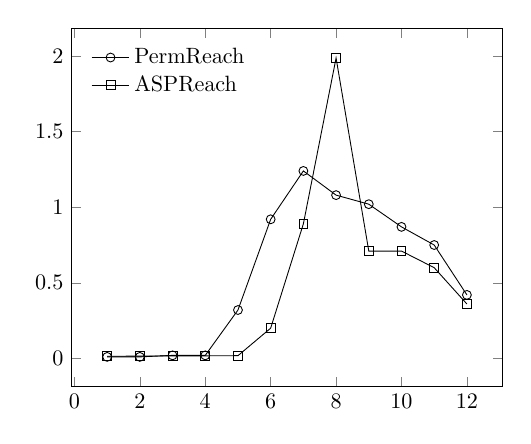
\begin{tikzpicture}[scale=0.8]
\begin{axis}%[legend style={at={(0,0)}, anchor=west,at={(axis description cs:0,-0.2)}}] 
\addplot[mark=o] coordinates {
        (1,0.01)
        (2,0.01)
        (3,0.02)
        (4,0.02)
        (5,0.32)
        (6,0.92)
        (7,1.24)
        (8,1.08)
        (9,1.02)
        (10,0.87)
        (11,0.75)
        (12,0.42)
    };
\addlegendentry{PermReach};
       \addplot[mark=square] coordinates{
        (1,0.014)
        (2,0.015)
        (3,0.017)
        (4,0.017)
        (5,0.018)
        (6,0.2)
        (7,0.89)
        (8,1.987)
        (9,0.710)
        (10,0.71)
        (11,0.6)
        (12,0.36)    
        };
        \addlegendentry{ASPReach}
\end{axis}
\end{tikzpicture}
\end{document}
